% !TEX root=../../mt-motion-analysis.tex
%!TeX spellcheck = en-US
\chapter{Methods}
\section{Overview}
In this chapter the system for assessing POEs will be presented. This system is naturally divided into two parts where firstly the videos are analyzed. The first subsystem extracts body part coordinates of the subjects. This information is then passed to the second subsystem where it is used to calculate a score according to \cite{Nae2017}. The data is presented in Section \ref{sec:met-data} and the two subsystems are described in Sections \ref{sec:met-loc} and \ref{sec:met-class} respectively.

\section{Data}\label{sec:met-data}
The data available is in the form of videos each containing one subject, recorded from the front, performing three-five repetitions of specific motions. The motions are \textit{Single-leg squat, Forward lunge, Stair descending, Forward lunge, Single leg hop for distance, and Side hop}. Each motion has a number of POE scores associated with them. The motion-POE combinations are shown in Table \ref{tab:met:motion-poes}. In Sections \ref{sec:met-SLS}-\ref{} the motions and POEs evaluated in this project are described.

% The videos were recorded with different orientations and frame rates.
%
% The available videos has been assessed by a physiotherapist and for each repetition in each motion a number of POE scores has been awarded.


\begin{table}
 \centering
 \caption{Motion-POE combinations available in the data.}
 \label{tab:met:motion-poes}

 \begin{tabular}{|c|ccccc|}
  \hline
  \backslashbox{POE}{Motion}                      &
  \multicolumn{1}{c}{\begin{tabular}[c]{@{}c@{}}Single\\ leg squat\end{tabular}}   &
  \multicolumn{1}{c}{\begin{tabular}[c]{@{}c@{}}Stair\\ descending\end{tabular}}   &
  \multicolumn{1}{c}{\begin{tabular}[c]{@{}c@{}}Forward\\ lunge\end{tabular}}   &
  \multicolumn{1}{c}{\begin{tabular}[c]{@{}c@{}}Single leg hop\\ for distance\end{tabular}}   &
  \multicolumn{1}{c|}{\begin{tabular}[c]{@{}c@{}}Side\\ hop\end{tabular}}                      \\ \hline \hline

  Trunk                                           & x & x &   & x & x \\ \hdashline
  Hip                                             & x & x & x & x & x \\ \hdashline
  \multicolumn{1}{|c|}{\begin{tabular}[c]{@{}c@{}}Femoral\\ valgus\end{tabular}} &
  x                                               & x & x & x & x     \\ \hdashline
  \multicolumn{1}{|c|}{\begin{tabular}[c]{@{}c@{}}Knee medial to\\ foot position\end{tabular}} &
  x                                               & x & x & x & x     \\ \hdashline
  \multicolumn{1}{|c|}{\begin{tabular}[c]{@{}c@{}}Femur medial\\ to shank\end{tabular}} &
  x                                               & x & x & x & x     \\ \hdashline
  Foot                                            & x &   &   &   &   \\ \hline
 \end{tabular}
\end{table}

bara skriva om sls? om det bara 'r sls jag bed;mt.. ocks[ skriva det som avgr'nsningar

\subsection{Single-leg squat, SLS} \label{sec:met-SLS}
The subject performed a squat standing on one leg to a knee angle of approximately $60\degree$. The exercise was repeated five times and the entire movement was used to assess the POEs \cite{Nae2020}. An illustration is shown in Figure \ref{}.

\subsection{Stair descending, SD}
The subject stepped down from a 30 cm step board. The exercise was repeated five times and POEs were evaluated for the loaded leg during loading phase \cite{Nae2020}. An illustration is shown in Figure \ref{}.

\subsection{Forward Lunge, FL}

Helo I am now mispealing.



% The data the system is designed for is in the form of videos each containing around five repetitions of some specific motion. For each repetition in each motion up to five POEs has been graded according to \cite{Nae2017}.


\section{Body part localization} \label{sec:met-loc}
% \subsection{Preprocessing}
% ...
% rotation, flip etc
% \subsection{Pose estimation}
%The pose estimation can be seen as a feature extraction and dimensionality reduction.
The pose estimation is built around the open-source toolbox MMPose \cite{mmpose} from MMLab. Each frame is considered to be an independent image and is analyzed with a \gls{hrnet} model with the \gls{dark} extension trained on the \gls{coco}-wholebody dataset\footnote{The model used can be found here: \url{https://mmpose.readthedocs.io/en/latest/top_down_models.html}.}. Both the model and the dataset is described in Section \ref{sec:pose_estimation}. % \ref{sec:hrnet, sec:dark, sec:coco}.

To get comparable results some of the videos were rotated and flipped before inferring the keypoints. This was needed since the videos were recorded in different orientations and the actions were performed with different legs. The rotations were based on the orientation of the subject (position of head w.r.t. the feet) in the first frame to have it standing up in the $y$-direction. Videos where the squats were performed with the left leg were then flipped around the $y$-axis to be able to use the same model for the left and right leg in a more efficient manner.

A bounding box for the subject is found using a Faster R-CNN model trained on the \gls{coco} dataset\footnote{The model used can be found here: \url{https://github.com/open-mmlab/mmdetection/tree/master/configs/faster_rcnn}.}. The content of this bounding box is resized to match the input size of the \gls{hpe} model used, 384$\times$288 pixels in our case. Each video analyzed results in sequences of $x$- and $y$-coordinates for all the keypoints in the dataset used to train the model.

%The file names contained information about which. The rotations were performed based on the position of the head with respect to the feet in the first frame.
\section{Classification} \label{sec:met-class}

\subsection{Preprocessing and dataset blabla..} \label{esc:met-class-preproc}
Before assessing the \glspl{poe} based on the body part positions a number of preprocessing steps are conducted. Firstly the data is resampled as the videos are recorded with a number of different frame rates ranging from 25 to 60 Hz. The resampling is performed using linear interpolation to a new sample frequency of 25Hz. This data is then low pass filtered through a fourth order Butterworth filter with a cutoff frequency of 2.5Hz. %PLOT P[ ;VERF;RING F;R FILTER? ELLER P[ FILTRERAD DATA?

While the \gls{poe} assessment, see Section \ref{sec:met-class-...}, is performed on a per repetition basis the body part coordinates are extracted on a per video basis. Hence, the sequences corresponding to the entire video is split up in the individual repetitions. This splitting algorithm is presented in Algorithm \ref{alg:rep} and is based on finding the edges of the peaks in specific position data. For the \gls{sls} task the $y$-coordinate of the right shoulder is used. The number of points extracted for each repetition depends on the width of the peak. The length of the observed repetitions varies from about 1 to 8 seconds. For practical reasons, such as handling of data and training performance\footnote{All data in one batch must have the same size. Hence, to be able to train with a batch size larger than 1, which usually improves training performance \cite{Goodfellow2016}, all data in the same batch needs to have the same dimensions.}, it is desirable to save the data as multidimensional arrays with the same dimensions. Two different ways of solving this problem is evaluated, namely i) padding the sequences and use maskings for the padded samples in the models, and ii) alternate the sample frequency to thereby achieve sequences of the same length.
%Some number of points around each peak is  This is done by finding peaks in the sequences corresponding to certain body part positions. Which body part is used for this sequence splitting depends on which movement is analyzed.

\begin{algorithm}
\SetAlgoLined
% \KwResult{Write here the result }
%  initialization\;
% peaks, right\_edges, left\_edges = \textbf{find\_peaks}(sequence)\;
right\_edges, left\_edges = \textbf{find\_edges}(sequence)\;
 \For{\textup{peak, right, current\_left, next\_left} in \textup{peaks, right\_edges, left\_edges}}{
 % \For{\textup{peak, right, current\_left, next\_left} in \textup{peaks, right\_edges, left\_edges}}{
  split\_index = \textbf{mean}(right, next\_left)\;
  start = \textbf{max}(current\_left - extra\_points, 0)\;
  end = \textbf{min}(right + extra\_points, split\_index)\;
  % start = \textbf{max}(peak - max\_length/2, 0)\;
  % end = \textbf{min}(peak + max\_length/2, split\_index)\;
  \textit{repetition} = \textbf{normalize\_length}(sequence[start:end])\;
  sequence = sequence[end:]\;
 }
 \caption{Extraction of repetitions from sequences}
 \label{alg:rep}
\end{algorithm}

%This is done by finding peaks in the time series corresponding to certain body part positions. Which body part is used for this sequence splitting depends on which movement is analyzed. For SLS the $y$-coordinate of the right shoulder is used. The duration of each repetition varies significantly. With the duration of each repetition varying substantially between subjects padding in the time dimension is desirable. The reason for this is twofold, i) to simplify the handling of the data by storing it as a multidimensional array, and ii) to be able to train the eventual model in a more efficient manner using batches \cite{Goodfellow2016}. The padding is done by adding constant values of -1000 at the end of the sequences to some specified length. Details on how this is handled by the model are presented in Section \ref{sec:met-class-model}


Finally the data is normalized. All coordinates are moved to put the mean position of the first five right hip-samples in the origin and are scaled to set the distance between the right shoulder and right hip to one, according to \eqref{eq:met-normalization}.

\begin{align}
  \begin{split}
    (x,y)_i &= (x,y)_i - {\mean{(x,y)}}_{rh} \\
    (x,y)_i &= \frac{(x,y)_i}{\lVert \mean{(x,y)}_{rs} \rVert_2} \qquad , \forall i
  \end{split}
  \label{eq:met-normalization}
\end{align}
\begin{conditions}
    $\mean{(x,y)}_i$  & =   & mean over first five samples for body part $i$ \\
    \textit{rh}     & =   & right hip \\
    \textit{rs}     & =   & right shoulder \\
    \textit{i}      & \in & Available body parts %\{body parts\}
\end{conditions}

After these preprocessing steps a dataset with inputs $\in \mathbb{R}^{N \times T \times F}$ and corresponding labels $\in \mathbb{Z}_3^N$ is created. The inputs consists of $N$ multivariate time series of length $T$ with $F$ channels. These channels are a subset of the extracted $x$- and $y$-coordinates as well as angles and differences between keypoints.

\subsection{Models}
For the modeling we evaluated some different deep learning based model architectures. The models eventually used were InceptionTime (Section \ref{sec:inception-time}) with different loss functions as well as an architecture designed by us, inspired by
\gls{xcm} (Section \ref{sec:XCM}) and InceptionTime. We call this model X-InceptionTime and it is presented below.

skriv om ensemble, vilka losses, maskning, icke maskning

\subsubsection{X-InceptionTime}
 The idea with this model was to combine the explainability of XCM with the inception module from InceptionTime. This was done by separating the inputs and having individual inception modules for each input channel as can be seen in Figure \ref{fig:x-inception}. After the final module (the depth can be seen as a hyperparamtere and needs to be tuned) a bottleneck of size one is applied reducing the dimensionality of each input channel back to $T$$\times$1. The features for the individual inputs are concatenated resulting in a feature map of size $T$$\times$$F$ where each input feature is only affected by that input. This makes it possible to use \gls{grad-cam} to see the importance of each time step for each input. Along with this it is also possible, thanks to the \gls{gap} layer, to get a measure of the importance of each input which can be used to reduce the dimensionality of the input.

 grad cam fr[n xinception

coral osv. custom losses osv?

\begin{figure}
  \centering
  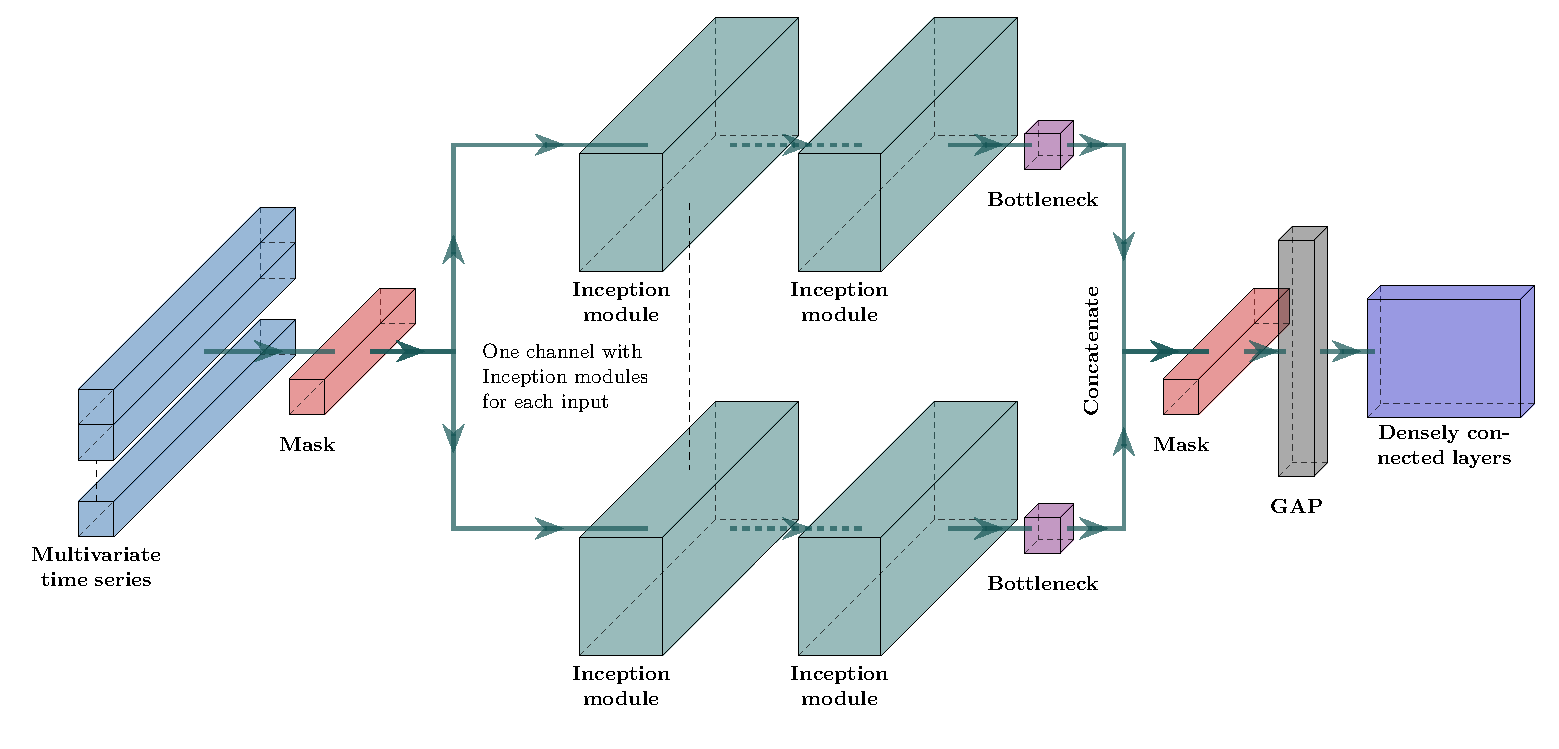
\includegraphics[width=\textwidth]{files/figs/x-inception.pdf}
  \caption{The X-InceptionTime architecture developed in this work.}
  \label{fig:x-inception}
\end{figure}

\subsection{Training}

\subsection{Choice of input features}

\subsection{Combined score}
